\lstdefinelanguage{cpp}{
%    backgroundcolor=\color{lgrey},  
    basicstyle=\footnotesize \ttfamily  \bfseries,   %\color{black}
    breakatwhitespace=false,       
    breaklines=true,               
    captionpos=b,
%    commentstyle=\color{dkgreen},   
    deletekeywords={...},          
    escapeinside={\%*}{*)},                  
%    frame=single,                  
    language=C++,                
 %   keywordstyle=\color{purple},  
%    morekeywords={size_t,string,void,int,gc_ptr,gc_new}, 
  %  identifierstyle=\color{black},
   % stringstyle=\color{blue},
 %   numbers=right,                 
 %   numbersep=5pt,                  
 %   numberstyle=\tiny, %\color{black}, 
%    rulecolor=\color{black},        
    showspaces=false,               
    showstringspaces=false,        
    showtabs=false,                
    stepnumber=1,                   
    tabsize=5
}

\title{Реализация основных примитивов\\ 
библиотеки неконсервативной\\
сборки мусора для C++}
%
\titlerunning{Реализация библиотеки сборки мусора для С++}
\author{Березун Даниил Андреевич}

%
\authorrunning{Д.А.Березун} % abbreviated author list (for running head)
%
%%%% list of authors for the TOC (use if author list has to be modified)
\tocauthor{Д.А.Березун}
%
\institute{Санкт-Петербургский государственный университет\\
\email{danya.berezun@gmail.com}}

\maketitle              % typeset the title of the contribution

\begin{abstract}
В работе описываются основные проблемы, возникающие при реализации точного сборщика для C++, приведена реализация 
такого сборщика мусора в виде пользовательской библиотеки, который не требует использования дружественного компилятора, 
но использует специализированную реализацию кучи. Также в работе подробно описаны и проанализированы соглашения на пользовательский код, 
необходимые для использование библиотеки, приведены примеры использования, и проанализированы накладные расходы, связанных 
с её использованием.
\end{abstract}

\section*{Введение}

Ручное управление памятью в языках, подобных C++, является источником большого количества трудно отслеживаемых ошибок, наличия которых можно было бы
избежать, сделав процесс управления памятью автоматическим. \textit{Сборка мусора} является одним из способов автоматического управления памятью, при
котором освобождение памяти выводится из-под контроля ПО на прикладном уровне. При автоматическом управлении программист не может явно влиять на распределение
объектов в памяти, у него есть лишь
косвенные способы сделать это с помощью использования тех или иных языковых конструкций. В идеальном случае, для рационального использования
памяти необходимо освобождать память, занимаемую объектами, которые более не будут использованы программой. Поскольку точно определить, что
объект не будет использован в дальнейшем, невозможно, на практике используют критерий доступности. \textit{Доступность} --- это консервативное
приближение используемости. \textit{Мусором}, в таком случае, называют объект, все пути доступа к которому уже разрушены, а память из-под него
ещё не освобождена. В некоторое, заранее определенное время, например, в простейшем случае, когда перестаёт хватать свободной памяти, выполнение
программы временно приостанавливается и запускается процесс \textit{сборки мусора}, который освобождает всю или ту, что возможно, память,
занятую мусором, после чего управление возвращается обратно программе. \textit{Сборщиком мусора} называется компонент, производящий \textit{сборку мусора}.

Процесс \textit{сборки мусора}, в простейшем случае, делят на три этапа:
\begin{enumerate}
\item \textit{Построение корневого множества}. На этом этапе строится множество объектов, которые считаются изначально доступными.
Такие объекты называются \textit{корнями} (англ. roots). Данное построение
аксиоматично, т.е. основывается на некотором наборе правил, согласно которым те или иные элементы считаются доступными. Данный этап является неотъемлемой
частью любого сборщика мусора.
\item \textit{Маркировка}. Начиная с множества, построенного на предыдущем этапе, происходит сканирование памяти, и все объекты, до которых возможно
добраться из построенного корневого множества, считаются доступными; оставшиеся объекты считаются мусором.
\item \textit{Освобождение}. Происходит сканирование кучи, в течение которого память из-под всех элементов, помеченных как мусор или не отмеченных как
доступные, освобождается.
\end{enumerate}

Есть несколько требований, которые должны быть выполнены для реализации сборки мусора:
\begin{enumerate}
\item Возможность построения корневого множества. Иными словами, необходимо иметь возможность идентифицировать все указатели в программном стеке, регистрах
и статической области памяти.
\item Должна присутствовать возможность определить все указатели из любого объекта на другие элементы кучи.
\end{enumerate}
В таких языках, как LISP или JAVA все условия соблюдаются, и в них успешно используется технология сборки мусора, в то время как, например,
в языке C не все условия выполняются. В языках, где не соблюдаются хотя бы одно из вышеперечисленных условий, возможна исключительна
\textit{консервативная сборка мусора}.
\textit{Консервативной} называется такая сборка мусора, при которой любой элемент данных, значение которого может быть истолковано, как указатель на
некоторый элемент кучи, считается  таковым. Консервативный подход к сборке мусора не позволяет собрать весь мусор, что может стать проблемой при обработке
большого количества данных. Неконсервативная сборка мусора лишена подобного недостатка и способна освободить всю память программы, более не
являющуюся доступной. \textit{Неконсервативным} или  \textit{точным сборком мусора} называется сборщик мусора, имеющий возможность точно распознать
все указатели в памяти. Иными словами, точный сборщик мусора --- это сборщик мусора, не использующий консервативный подход.

В C++ не соблюдаются требования, необходимые для сборки сборки мусора, реализовать точный сборщик мусора без ограничений
на использование некоторых примитивов языка не представляется возможным.
Более того, в C++ имеется ряд технических сложностей, затрудняющих реализацию точного сборщика мусора.
Тем не менее, в случае соблюдения программистом некоторых соглашений на програмный код,
точная сборка мусора становится возможной и в C++.

Целями работы является реализация основных примитивов библиотеки неконсервативной сборки мусора для C++,
обеспечение возможности совмещения ручного и автоматического управления памятью.

Когда говорят об управлении памятью, часто употребляют термин \textit{автоматический объект}.
Зачастую так переводят два различных английских термина: \textit{automatic object} и \textit{managed object} (или
\textit{managed memory}).

Automatic object --- объект, который автоматически выделяется и удаляется, при входе/выходе программного потока в/из контекста.

Managed object --- объект, автоматически управляемый менеджером памяти.

Во избежание путаницы в данной работе используются термины \textit{стековый объект} для automatic object
и \textit{управляемый объект} для managed object.

\section{Обзор}

Для C++ существует несколько применяемых подходов к реализации сборки мусора.
Их принято разделять на три основных класса\cite{CppArt}:
\begin{enumerate}
\item консервативный подход;
\item подходы, основанные на ``умных'' указателях;
\item введение новых примитивов, используемых для организации ссылок на автоматически управляемую память.
\end{enumerate}
Описание каждого из вышеизложенных подходов приведено далее в соответствующих подчастях.

\subsection{Консервативный подход}
Консервативный подход заключается в том, что, не имея возможности точного выявления указателей в памяти программы,
указателем считается любое значение в памяти, которое может таковым являться.
Одной из основных задач при реализации консервативного сборщика мусора является разработка алгоритмов
и/или критериев, согласно которым принимается решение о том, является то или иное значение в памяти указателем,
или же оно случайным образом попадает в диапазон адресов кучи.

Наиболее популярным сборщиком мусора для С++ является BoehmGC\footnote{\texttt{http://www.hboehm.info/gc/}}.
Он использует именно консервативный подход к сборке мусора.
BoehmGC подменяет функции работы с памятью на аналогичные, реализованные его разработчиками,
сохраняя метаинформацию о выделяемых объектах.
При идентификации указателей в памяти одним из тестов на их легитимность является проверка
на то, совпадает ли конретное значение со значением указателя, полученного как результат
выделения памяти, и существует ли метаинформация, ему соответствующая.
Одной из основных причин использования BoehmGC консервативного подхода является тот факт,
что подобный подход накладывает минимальные ограничения на пользовательскую программу.
Одной из целей, которой придерживаются разработчики BoehmGC, является совместимость с уже существующими
программами, написанными на C++, без внесения каких-либо изменений в их исходный код\cite{BoehmTransGC}.
BoehmGC может использоваться не только в качестве сборщика мусора, но и как детектор утечек памяти в программе.

Основным недостатком консервативных сборщиков мусора является отсутствие возможности идентификации
всего скопившегося мусора. Чем больше данных обрабатывает программа, тем больше вероятность случайного совпадения
какого-то значения в памяти со значением указателя. Поэтому при обработке большого количества данных
консервативность сборщика мусора может стать проблемой, которая может привести к исчерпанию памяти,
которого могло бы не произойти, будь собран весь скопившейся мусор.
Конечно, в подобной ситуации не всегда происходит исчерпание памяти, однако большое количество несобранного мусора
может повлечь за собой неоправданные задержки в работе самого сборщика мусора.

\subsection{``Умные'' указатели}
``Умный'' указатель (smart pointer) --- это класс, реализующий интерфейс указателя, предоставляющий некоторую
дополнительную функциональность.
``Умные'' указатели способны облегчить процесс управления динамической памятью, при условии их правильного использования,
однако не являются панацеей, позволяющей избежать всех проблем управления памятью в C++\cite{smartPointers}.

Некоторые из ``умных'' указателей реализуют программную идиому RAII (Resource Acquisition Is Initialization).
Смысл RAII заключается в том, что использются некоторые механизмы, неразрыно связывающие получение ресурса с его инициализацией,
а освобождение --- с уничтожением объекта. Зачастую ``умные'' указатели, использующие RAII, представляют собой классы,
инкапсулирующие владение памятью. Подробнее про RAII можно прочитать в \cite{CppPrinciples}.
Одним из представлителей подобного подхода является \lstinline[language= cpp]{auto_ptr}.
\lstinline[language= cpp]{auto_ptr} использует семантику разрушающего копирования, что не позволяет использовать его
в контейнерах стандартной библиотеки\cite{smartPointers}.
Существуют и более универсальные ``умные'' указатели, такие как \lstinline[language= cpp]{shared_ptr},
реализующий совместное владение объектом, и \lstinline[language= cpp]{weak_ptr} представляющим собой указатель,
не владеющий экземпляром объекта.
Для реализации совместного влядения \lstinline[language= cpp]{shared_ptr} использует алгоритм \textit{подсчёта ссылок}.
Подсчёт ссылок заключается в том, что у каждого объекта есть счётчик, называемый \textit{счётчиком ссылок},
значение которого увеличивается на единицу
при появлении очередной ссылки на объект, и уменьшается на неё же, при разрушении какой бы то ни было ссылки на этот объект.
Как только счётчик ссылок становится равным нулю, это означает, что на объект более никто не ссылается и его можно удалить.

Существует множество ``умных'' указателей, использующих подсчет ссылок для определения времени жизни объекта:
\lstinline[language= cpp]{boost::intrusive_ptr, boost::scoped_pt, boost::scoped_array<>, boost::shared_array<>},
также существуют реализации в библиотеках Loki\cite{Alexandrescu}, Poco\footnote{\texttt{http://pocoproject.org/}} и многих других.
Основным преимуществом алгоритма посчёта ссылок является простота его реализации и понимания программистом.
Камнем же преткновения вышеописанного алгоритма является выявление \textit{циклических ссылок}, т.е. когда два объекта
напрямую или косвенно ссылаются друг на друга. В случае возникновения циклических ссылок, счётчик ссылок никогда не обнулится,
и память не будет освобождена, даже если объекты, связанные циклическими ссылками, уже не являются доступными.
Сами по себе ``умные'' указатели не решают проблемы выявления циклических ссылок, возлагая ответственность на программиста.
При реализации сборщика мусора, основанного на использовании ``умных'' указателей с алгоритмом подсчёта ссылок,
реализация детектора циклических ссылок является одной из основных и нетривиальных задач.
Конечно, существуют алгоритмы обнаружения циклических ссылок, однако время, затрачиваемое на их обнаружение,
зачастую не оправдывает их использование.

\subsection{Введение дополнительных примитивов}
Данный подход к сборке мусора заключается в введении нового примитива в язык, подобно ``умному'' указателю,
представляющего собой ссылку в автоматически управляемую память, и предоставления функции выделения автоматически управляемой
памяти под введенный примитив.
Основным преимуществом такого подхода является возможность реализации точной сборки мусора с использованием различных алгоритмов.
Именно этого подхода и придерживается реализуемая библиотека сборки мусора.
Одним из сборщиков мусора, реализующих подобный подход, является GC++\footnote{\texttt{http://gcplusplus.sourceforge.net/classGCpp\_1\_1gc\_\_ptr.html}}. В силу своей простоты он имеет ряд ограничений, которых можно было бы избежать.
Так, например, в нём не поддерживаются массивы и множественное наследование в силу особенностей реализации.

Основными недостаткоми данного подхода являются следующие:
увеличение времени исполнения кода по сравнению с ручным управление памятью
и использование большого количества памяти для хранения метаинформации.
Однако подобными недостатками в той или иной степени обладают все подходы к сборке мусора в C++.

\section{Реализация}

Существует множество алгоритмов сборки мусора, однако одним из наиболее популярных является алгоритм пометки и освобождения
(англ. mark-and-sweep) и его вариации. Популярность данного алгоритма связана с минимальным количеством ограничений,
накладываемых на язык и сборщик мусора, и простотой самого алгоритма. Всё, что необходимо для его реализация ---
возможность построить корневое множество, уметь идентифицировать ссылки внутри объекта и иметь возможность
каким бы то ни было способом помечать объекты как живые. Данный алгоритм используется и во многих консервативных
сборщиках мусора, просто в таких случаях реализуемый сборщик мусора не является точным.
В классической реализации алгоритм пометки и освобождения является алгоритмом \textit{с полной остановкой мира}
(англ. stop-the-world),
иными словами, пользовательская программа прерывается на время работы сборщика мусора и продолжается после её окончания.
В предлагаемой работе будет использоваться именно вышеуказанный алгоритм. На то есть две основные причины:
во-первых, выбор конкретного алгоритма сборки мусора не является самоцелью данной работы,
во-вторых, предлагаемая реализация библиотеки сборки мусора предусматривает возможность дальнейшей реализации
широкого множества алгоритмов сборки мусора, как сжимающих или перемещающих, так и сборщиков мусора с
поколениями~\cite{GCHandbook}.

Как уже упоминалось ранее, используемый алгоритм сборки мусора делится на три фазы: построение корневого множества,
маркировку живых объектов, освобождение памяти. Реализация каждой фазы сборки мусора преставляет собой
ряд нижеописанных задач, подробное решение каждой из которых будет приведено в соответствующей части данной работы.

Для построения корневого множества необходимо решить, каким образом будет это корневое множество формироваться:
автоматически во время исполнения программы или же путем сканирования памяти
во время работы самого сборщика мусора, а также где и в каком виде хранить сами корни.
Для поиска корневых объектов нет необходимости сканировать всю память программы, достаточно ограничиться
программным стеком, регистрами и статической областью памяти~\cite{myCoursePaper}.
Для маркировки объекта необходимо иметь хотя бы один свободный бит в его заголовке или реализовывать некую структуру,
хранящую информацию о марке каждого объекта. Последнее решение является чрезмерно неэффективным по памяти, поэтому,
как правило, не используется. Существует несколько известных алгоритмов маркировки объектов:
\begin{enumerate}
\item \textit{Однобитная маркировка}. Выставляется один бит маркировки в заголовке объекта.
\item \textit{Трехцветная маркировка}. Выставляется два бита в заголовке объекта, говорящих о ``цвете'' объекта:
	\begin{enumerate}
	\item Белый. Означает, что объект ещё не был помечен. Изначально все объекты, кроме корней, белые.
	\item Серый. Означает, что объект уже помечен, но некоторые ссылки из него ещё не помечены. Корневое множество
		изначально серого цвета.
	\item Чёрный. Объект помечен, из него не осталось ссылок на белые объекты.
	\end{enumerate}
Существует несколько вариаций алгоритма трёхцветной маркировки, все они используются
исключительно для осуществления \textit{корнкурентной} маркировки объектов, т.е. маркировки объектов одновременно
с исполнением самой программы. Конкурентная маркировка используется для минимизации stop-the-world паузы.
\end{enumerate}
В реализумом сборщике мусора используется однобитная маркировка.
Реализация трехцветной маркировки является одним из возможных путей дальнейшего улучшения библиотеки.
Дополнительные биты в заголовке объекта появляются ввиду подмены стандартной кучи, используемой стандартным
\lstinline[language= cpp]{malloc} и \lstinline[language= cpp]{new}, на кучу Дага Ли.

\subsubsection{Malloc Дага Ли и его использование в сборщике мусора.}

Malloc Дага Ли (Doug Lea's Malloc)\footnote{\cd{ftp://g.oswego.edu/pub/misc/malloc.c}}
представляет собой реализацию кучи, на основе которой
написан ptmalloc, используемый в библиотеке glib (GNU C library). Память кучи распределяется по сегментам (chunks), имеющим
восьмибайтовое выравнивание, содержащим заголовок и свободную память. Каждый блок памяти имеет свою метаинформацию в размере
8 или 16 байт, содержащую флаги, размер блока и указатели на предыдущий и последующий элементы (boundary tags),
сами же сегменты связаны по их размеру (см. рис.~\ref{boundary_tags} и \ref{bindings}).

\begin{figure}[t]
  \centering
  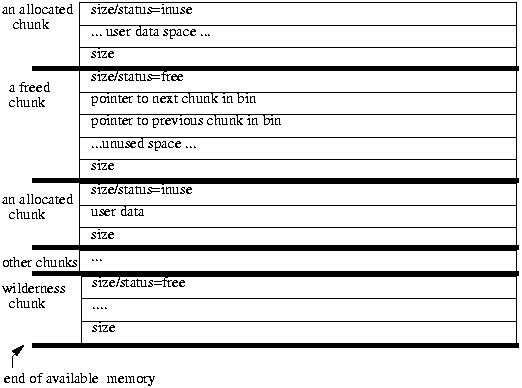
\includegraphics[width=\linewidth]{Berezun/images/boundaryTags.png}
  \caption{malloc Дага Ли: boundary tags}
  \label{boundary_tags}
\end{figure}

\begin{figure}[t]
  \centering
  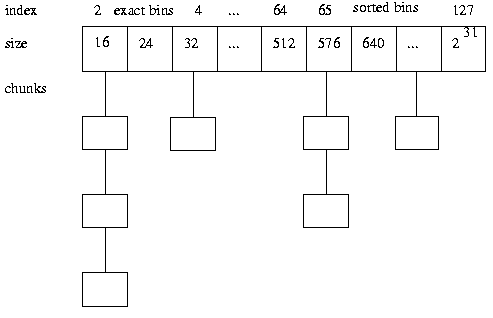
\includegraphics[width=\linewidth]{Berezun/images/binding.png}
  \caption{malloc Дага Ли: сегменты}
  \label{bindings}
\end{figure}

Куча Дага Ли позволяет эффективно решать задачу освобождения неиспользуемой памяти.
Очевидно, что освобождение памяти извне программной кучи требует хранение дополнительной иформации о блоках памяти,
ставших мусором, и нетривиальную реализацию обхода этих блоков с целью освобождения, время которого будет весьма
чувствительно к внутреннему устройству кучи и алгоритмам освобождения памяти в ней.
Сама же куча могла бы сделать массовое освобождение памяти, а именно такое освобождение памяти происходит при сборке мусора,
куда более рационально, используя различные алгоритмы~\cite{GCBook1}
и руководствуясь стратегией(-ями), которой данная реализация кучи придерживается.
Куча может вообще отложить часть работы по освобождению памяти до более подходящего времени,
исходя из принципа минимизации stop-the-world-паузы.
К счастью, существует модификация кучи Дага Ли,
предоставляющая эффективную функцию массового освобождения памяти~\cite{msmalloc}.
Более того, и нижесказанное является одной из основных причин использования кучи Дага Ли,
\lstinline[language= cpp]{dlmalloc} имеет бит маркировки в заголовке каждого сегмента. Совместно с функцией массового освобождения
памяти \lstinline[language= cpp]{dlmalloc} представляет собой готовую инфраструктуру для реализации сборки мусора.

Для обеспечения возможности совмещения ручного и автоматического управления памятью и маркировки объектов
реализованному сборщику мусора необходимо иметь два свободных бита в заголовке каждого объекта:
один бит для маркировки объекта, второй --- для флага, говорящего, является объект
управляемым или ``ручным''.
Куча Дага Ли при сборке в 64-x битной
системе ввиду выравнивания в заголовке объекта остаётся дополнительный свободный бит, который можно использовать.
Т.о. при сборке кучи в 64-x битной системе в заголовке объекта образуется один свободный бит
и бит маркировки, т.е. два бита, как того и требовалось.
Использование 64-x битной системы в данном случае чрезвычайно важно,
поскольку в 32-х битной версии дополнительного свободного бита нет. В последнем случае остаётся возможность
обеспечить сборку мусора, но для совмещения ручного и автоматического управления памятью необходимо было бы прибегнуть к
иным решениям. Ввиду вышесказанного использование 64-x битной системы является одним из ограничений
использования реализуемой библиотеки сборки мусора.
Немного подробнее об использовании двух битов в заголовке объекта для маркировки и совмещения ручного и автоматического
управления памятью:
\begin{enumerate}
\item По умолчанию аллокатор выставляет значение обоих битов в 0. Значение 0 первого бита означает, что объект ``ручной''.
\item При использовании примитивов самой библиотеки сборки мусора (ф-ия \lstinline[language= cpp]{gc_new} для выделения памяти),
	значение первого бита меняется на 1, что означает, что объект является управляемым.
\item Второй бит является битом маркировки: 0 --- объект не помечен, 1 --- объект помечен --- для управляемых
	объектов и не имеет никакого значения для ``ручных''.
\end{enumerate}
Т.о. достигается возможность совмещения ручного и автоматического управления памятью.
Разумеется, возникает проблема наличия ссылок из ручных объектов на управляемые,
подробное описание возникшей задачи и её решение расположено в части.

\subsubsection{Функции mmap и munmap}
Для работы с памятью, используемой для реализации сборщика мусора, используются следующие функции, позволяющие
работать с памятью вне программной кучи и стека, что позволяет избежать сборки мусора в самом сборщике мусора:
\begin{enumerate}
\item \lstinline[language= cpp]{void *mmap (void *, size_t, int, int, int, off_t)}\footnote{\cd{http://man7.org/linux/man-pages/man2/mmap.2.html}}
	для выделения памяти.\\*Функция принимает в качестве аргументов (слева направо):
	\begin{enumerate}
	\item желаемый адрес начала участка отбраженной памяти, если 0 --- ядро само выберет адрес;
	\item количество байт, которое нужно отобразить в память;
	\item число, определяющее степень защищённости отображенного участка памяти (только чтение, только запись, исполнение, область
		недоступна);
	\item атрибуты области;
	\item дескриптор файла, который нужно отобразить;
	\item смещение отображенного участка от начала файла.
	\end{enumerate}
	и возвращает адрес начала участка отображаемой памяти или \lstinline[language= cpp]{MAP_FAILED} в случае неудачи.
\item \lstinline[language= cpp]{int munmap (void *addr, size_t length)} для освобождения памяти.
	Параметр addr является адресом начала области памяти, выделенной для отображения файла, т.е. значением, которое вернул системный вызов \lstinline[language= cpp]{mmap}, параметр length определяет ее длину и его значение должно совпадать со значением соответствующего параметра в системном вызове \lstinline[language= cpp]{mmap}. При нормальном завершении системный вызов возвращает значение 0, при возникновении ошибки --- значение -1.	
\end{enumerate}

\subsection{Общая архитектура библиотеки сборки мусора}
На пользовательском уровне существует два основных примитива библиотеки:
\begin{enumerate}
\item ``Умный'' указатель \lstinline[language= cpp]{gc_ptr<class_name>}. Представляет собой ``умный'' указатель на объект типа
	\lstinline[language= cpp]{class_name}.
	Данный примитив предлагается как альтернатива для указателей языка, являющаяся основой для идентификации ссылок из
	обного объекта на другой и построения корневого множества.
\item Функция выделения памяти \sloppy\lstinline[language= cpp]{<constructor_argument_types, allocation_object_type> gc_new (constructor_arguments, array_count = 1)}. Данный примитив используется для выделения автоматически управляемой памяти под объект типа \lstinline[language= cpp]{allocation_object_type} с помощью вызова конструктора объекта, имеющего типы параметров такие же и следующие в том же порядке, что передаются функции в списке \lstinline[language= cpp]{constructor argument types};
	\lstinline[language= cpp]{constructor_arguments} --- соответствующие перечисленным типам значения;
	\lstinline[language= cpp]{array_count} --- количество элементов массива, при выделении массива объектов типа
	\lstinline[language= cpp]{allocation_object_type}, по умолчанию равно 1, что означает выделение одиночного объекта.
\end{enumerate}
При использовании вышеуказанных примитивов следующим образом: \lstinline[language= cpp]{gc_ptr} вместо указателей языка и
\lstinline[language= cpp]{gc_new} в качестве единственной функции выделения памяти --- утверждается,
что управление памятью является автоматическим, а сборка мусора --- точной.

Связь между объектами системы представлена на рис.~\ref{fig:systemArch}. Подробное описание каждого компонента системы предоставлено
ниже в соответствующих частях.

\begin{figure}[t]
	\centering
	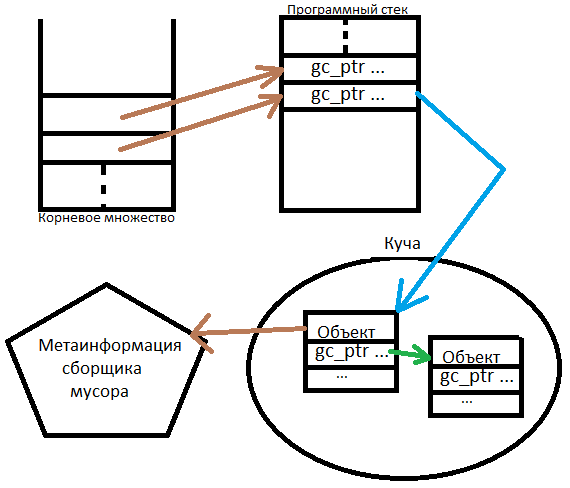
\includegraphics[width=0.8\linewidth]{Berezun/images/systemArch.png}
	\caption{Системные и пользовательские данные}
	\label{fig:systemArch}
\end{figure}

\subsection{Представление корней}
От того, каким образом хранятся корни, и насколько сложны операции поиска, удаления и добавления нового элемента,
напрямую зависит скорость выполнения фазы маркировки объектов и построения корневого множества.
В реализуемой библиотеке сборки мусора построение корневого множества происходит во время исполнения программы
следующим образом: при загрузке стековой рамки на стек все стековые объекты,
являющиеся \lstinline[language= cpp]{gc_ptr}, в своём конструкторе вызывают функцию добавления себя в корневое множество;
при вытеснении стековой рамки со стека эти же объекты вызывают функцию удаления себя из списка корневых объектов
в своём деструкторе; статические объекты, являющиеся \lstinline[language= cpp]{gc_ptr}, добавляются в корневое множество
в момент инициализации статической области и не удаляются оттуда в течение всего времени жизни программы.
Такой подход к построению корневого множества, разумеется, имеет свои минусы: при каждой загрузке/выгрузке
стековой рамки на/с вершину стека корневое множество будет меняться, образуя некоторую
задержку в исполнении программы. В случае, если между запусками сборки мусора есть значительное количество операций
над стеком, изменения корневого множества могут происходить впустую. Рис.~\ref{fig:stackLive} иллюстрирует вышеизложенную мысль
на конкретном примере более наглядно: предположим, что между двумя соседними запусками сборки мусора было множество
операций загрузки/выгрузки стековых рамок, а сам стек остался таким же; корневое множество менялось при каждой такой
операции, но осталось при этом неизменным.

\begin{figure}[t]
	\centering
	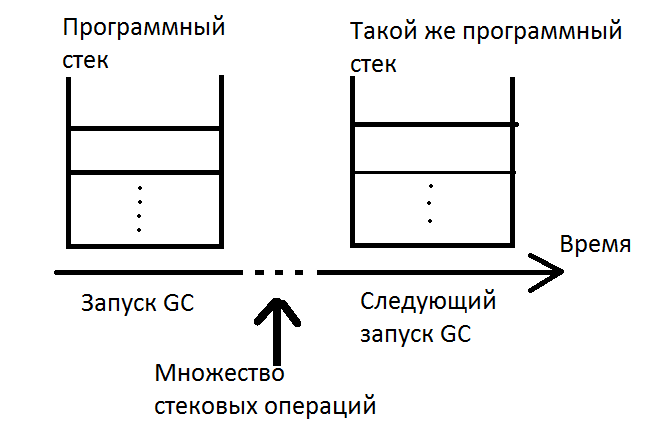
\includegraphics[width=0.7\linewidth]{Berezun/images/picture1.png}
	\caption{Пример стека при соседних запусках сборщика мусора}
	\label{fig:stackLive}
\end{figure}

Построение корневого множества исключительно в момент запуска самой сборки мусора
изменяло бы корневое множество лишь единожды, однако такое построение требует нетривиальной идентификации корней
в программном стеке, что может привести к долгосрочной паузе в исполнении программы, и не может являться
точным, поскольку невозможно в точности распознать все объекты определенного типа в программном стеке, не
внедряясь в компилятор, из-за возможности совпадения случайного значения в стеке с искомым объектом. Подобное
построение всегда консервативно.

Для решения задачи миниизации времени работы операций над корневым множество было предложено следующее решение:
\begin{enumerate}
\item Cтруктура для хранения корней представляет собой стек.
Согласно стандарту C++-11\footnote{\cd{https://isocpp.org/std/the-standard}} деструкторы стековых объектов вызываются в порядке, обратном вызову
их конструкторов, поэтому использование стека обусловлено быстротой выполнения операций вставки и удаления элементов.
Т.о. для удаления из корневого множества объекта достаточно произвести простой декремент указателя на вершину стека.
\item Стек представляет собой пул памяти.
Во избежание излишних затрат времени на маркировку самого корневого множества, которая вызывалась бы при каждом срабатывании
сборщика мусора, корневое множество реализовано не в программной куче, а в отдельном пуле памяти. Т.о. в фазе освобождения
памяти корневое множество не будет затронуто вовсе, а соответственно, и маркировка ему в таком случае не нужна,
что позволяет избежать хранения метаинформации для корневого множества, тем самым экономя память.
Сам же пул представляет собой динамическую область памяти, выделяемую с помощью функции \lstinline[language= cpp]{mmap}.
\item Стек реализован с использованием шаблона объектного проектирования singleton~\cite{patterns}.
Т.о. достигается уникальность корневого множества.
\end{enumerate} 

\begin{figure}[t]
	\centering
	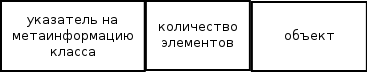
\includegraphics[width=0.6\linewidth]{Berezun/images/objectMeta.png}
	\caption{Метаинформация, хранимая рядом с объектом}
        \label{metainfo}
\end{figure}

\begin{figure}[t]
	\centering
	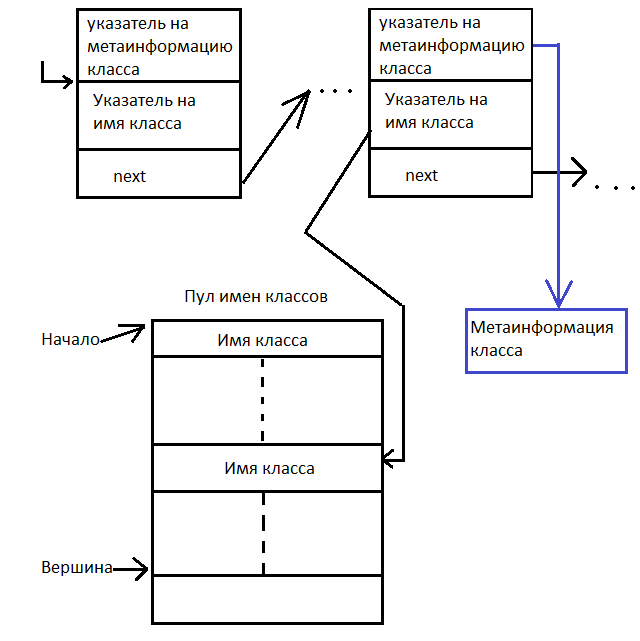
\includegraphics[width=0.9\linewidth]{Berezun/images/picture2.png}
	\caption{Представление метаинформации}
        \label{metarepr}
\end{figure}

\subsection{Представление метаинформации}
Метаинформация в данной реализации сборщика мусора бывает двух типов: хранимая рядом с объектом и метаинформация для каждого класса, объект которого был хотя бы раз создан в куче.
Метаинформация, хранимая рядом с объектом, представляет собой простой указатель на метаинформацию класса,
которому данный объект принадлежит, и значение типа \lstinline[language= cpp]{size_t},
хранящего количество элементов массива, если объект представляет собой массив, 0 --- иначе.
Данный тип метаиформации расположен в памяти непосредственно перед самим объектом и имеет фиксированный размер (см. рис.~\ref{metainfo}).

Основной задачей, решаемой хранением метаинформации, является возможность обхода графа живых объектов на стадии маркировки,
начиная с корней. Происходит это следующим образом: по объекту находится метаинформация класса, которому он принадлежит;
в этой метаинформации хранятся смещения \lstinline[language= cpp]{gc_ptr} на другие объекты кучи относительно начала
самого объекта; функция маркировки запускается ото всех объектов, на которые ссылаются указатели,
лежащие на заданных смещениях от начала самого объекта.
Для поиска метаинформации класса, которому принадлежит объект, достаточно перейти по указателю, лежащему в метаинформации
объекта непосредственно перед ним.
Сама метаинфомация класса вычисляется в момент создания первого объекта подобного типа и заносится в список пар
<имя класса, его метаинформация>. Метаинформация класса (см. рис.~\ref{metarepr}) представляет собой специальным образом хранимые смещения
указателей на другие элементы класса от начала объекта. У всех объектов одного типа смещения от начала объекта до его полей
неизменны, что и позволяет высчитать их для каждого класса лишь единожды.
Подробнее об этом процессе можно прочитать в работе~\cite{kren}.

Метаинформация класса бывает двух типов:
\begin{enumerate}
\item \lstinline[language= cpp]{box_simple} --- для простых объектов и массивов \textit{простых объектов},
	т.е. объектов, не содержащих ссылок в кучу. Представляет собой просто метку о том, что объект не содержит ссылок на другие
	объекты кучи.
\item \lstinline[language= cpp]{generic_box_struct} --- для объектов, имеющих ссылки в кучу внутри себя.
	В памяти подряд хранятся структуры, каждая из которых хранит смещение объекта до очередной ссылки из него и бит,
	говорящий о том, является ли данная ссылка ссылкой на простой объект или же нет.
\end{enumerate}
Структура для хранения метаинформации представляет собой список пар <указатель на имя класса, указатель на метаинформацию класса>,
для краткости далее будем называть этот список просто \textit{список метаинформации классов}.
Имена классов хранятся подряд в отдельном пуле памяти, вычисляются с помощью шаблонов C++ с использованием
функции \lstinline[language= cpp]{typeid} в момент выделения памяти под объект.
Подобное представление позволяет хранить исключительно имена классов без какой-либо дополнительной метаинформации о них
или реализации специальных структур данных, что, несомненно, экономит память программы.
Очевидно, что предложенная реализация затрудняет поиск элемента в пуле и его удаление, однако
операций поиска и удаления элементов из пула памяти с именами классов не происходит, потому что метаинформация,
будучи единожды созданной для класса, уже не удаляется, т.к. всегда может понадобиться в дальнейшем, соответственно
и имя класса также необходимо хранить. Поиск элемента в пуле для имен классов также не происходит,
поскольку для любого имени класса существует запись в списке метаинформации классов, в котором и происходит
поиск метаинформации класса при создании объекта с помощью функции \lstinline[language= cpp]{gc_new}.

\subsection{Совмещение ручного и автоматического управления памятью}

Как уже говорилось, пользователю предоставляется возможность совмещения автоматического и ручного управления памятью,
в связи с чем возникает следующая проблема: наличие ссылки из ручного на управляемый объект.
В случае, если более не осталось ссылок из управляемых объектов на данный объект, а из ручного на него ссылка есть,
сборщик мусора удалит рассматриваемый объект, и ссылка станет висячей.
Предлагается следующее решение данной проблемы: предоставить пользователю функцию регистрации и дерегистрации управляемого объекта
как \textit{мнимого корня}, т.е. объекта, который приравнивается к корневым, хотя таковым не является.
Поскольку порядок регистрации и дерегистрации объекта, как мнимого корня, никак не определен и происходит исключительно по 
желанию пользователя, оптимизировать их хранение столь же эффективно, как хранение обычных корней, не представляется возможным,
в связи с чем все мнимые корни хранятся в отдельной древовидной структуре, хранимой в куче.

Конечно, такой подход небезопасен, поскольку, в случае ошибки пользователя, могут возникнуть висячие ссылки, или появиться 
несобираемый мусор, если пользователь забудет дерегистрировать объект.
Но, стоит заметить, что возникновение ошибок подобного рода никоим образом нельзя избежать при ручном управлении памятью.

\section{Ограничения}

Предлагаемая реализация библиотеки сборки мусора использует функцию \lstinline[language= cpp]{mmap} для выделения памяти в
вируальном адресном пространстве. Подобное решение может использоваться лишь в UNIX-системах.
В ОС Windows существует функция \lstinline[language= cpp]{VirtualAlloc()}, предоставляющая требуемую функциональность.
Тем не менее, этого недостаточно для обеспечения переносимости сборщика мусора на ОС Windows.
Используемая в реализации куча Дага Ли, по словам самого автора\footnote{\cd{http://g.oswego.edu/dl/html/malloc.html}},
гарантирует правильность работы только на UNIX-подобных системах.
Проверки на совместимость с ОС Windows автором работы не проводилась.

Ещё одним уже упоминавшемся ограничением использования предлагаемой реализации является 64-х битная версия системы.
Как уже говорилось, работа сборщика мусора в 32-х битной системе возможна, но без предоставления возможности
совмещения ручного и автоматического управления памятью.

\section{Примеры}
%http://hboehm.info/gc/gc\_bench/GCBench.cpp
В данной части работы приведены примеры использования реализованной библиотеки неконсервативной сборки мусора.

\subsection{Совмещение ручного и автоматического управления памятью}
Здесь приведен простой пример совмещения автоматического и ручного управления памятью,
демонстрирующий принцип написания подобного кода.
Код подробно прокомментирован.

\begin{lstlisting}[language=cpp, mathescape=true]
# include <libgc/libgc.h>
# include <iostream>

struct str2 {
  gc_ptr<int> p;
};

struct str1 {
  gc_ptr<str2> p;
};

int main (void) {
  /// $\mbox{Выделение памяти под ``ручной'' объект типа str1}$
  str1 * s = (str1 *) malloc (sizeof(str1));

  /// $\mbox{Выделение управляемой памяти под управляемый объект}$
  /// $\mbox{внутри ``ручного''}$
  s->p = gc_new<str2>();

  /// $\mbox{Вызов функции register\_object,}$
  /// $\mbox{сообщающей сборщику мусора,}$
  /// $\mbox{что на управляемый объект,}$
  /// $\mbox{расположенный в памяти по адресу}$
  /// $\mbox{\&(s->p), появилась дополнительная ``внешняя'' ссылка}$
  register_object(&(s->p));

  /// $\mbox{Выделение управляемой памяти под управляемый массив}$
  s->p->p = gc_new<int>(1000);
  
  /// $\mbox{Принудительный вызов сборки мусора.}$
  /// $\mbox{После выполнения данной функции}$
  /// $\mbox{ни один выделенный объект}$
  /// $\mbox{не должен быть удален, т.к.}$
  /// $\mbox{объект s --- ручной,}$
  /// $\mbox{объект s->p --- управляемый,}$
  /// $\mbox{на который существует ссылка из ручного,}$
  /// $\mbox{объект s->p->p --- управляемый,}$
  /// $\mbox{на который существует ссылка}$
  /// $\mbox{из автоматического, достижимого из ``ручного''}$
  mark_and_sweep();
  
  /// $\mbox{Сообщение сборщику мусора о том, что на объект,}$
  /// $\mbox{лежащий по адресу \&(s->p) одна из ссылок из}$
  /// $\mbox{``ручных'' объектов более не требуется}$
  unregister_object(&(s->p));
  s->p = NULL;
  
  /// $\mbox{Принудительный вызов сборки мусора.}$
  /// $\mbox{После выполнения данной функции объекты}$
  /// $\mbox{s->p и s->p->p должны быть удалены.}$
  mark_and_sweep();
  
  /// $\mbox{Вызов функции transfer\_to\_automatic\_objects(void * s)}$
  /// $\mbox{переводит ``ручной'' объект, расположенный по адресу \&s,}$
  /// $\mbox{в управляемые.}$
  /// $\mbox{Фактически это означает, что объект s более не нужен}$
  /// $\mbox{пользователю и его можно удалить}$
  /// $\mbox{во время ближайшей сборки мусора}$
  transfer_to_automatic_objects(s);
  
  /// $\mbox{Принудительный вызов сборки мусора.}$
  /// $\mbox{После выполнения данной функции объект}$
  /// $\mbox{s должен быть удален.}$
  mark_and_sweep();

  return 0;
}
\end{lstlisting}

\subsection{АВЛ-дерево}
Данный пример представляет собой реализацию АВЛ-дерева.
Нетрудно заметить, что код, приведенный ниже, представляет собой ``обычный'' код на C++, где
изменились лишь функции выделения памяти, заменены указатели C++ на \lstinline[language= cpp]{gc_ptr}
и опущены функции освобождения памяти.

\lstinputlisting[language=cpp]{Berezun/codes/avl_with_gc.cpp}

Затраты на сборку мусора на данном примере замедляют работу программы примерно на порядок.

\section*{Заключение}

В данной работе было предложено решение задачи реализации неконсервативной сборки мусора для языка C++,
а также описаны соглашения, накладываемые сборщиком мусора на программный код.
Предложенные соглашения не накладывают каких-либо функциональных ограничений на язык.

Существует несколько направлений для дальнейшего развития данной работы:
\begin{enumerate}
\item усовершенствование процесса сборки мусора за счёт использования алгоритмов, отличных от mark-and-sweep;
\item изменение стратегии массового освобождения памяти кучей Дага Ли в целях минимизации stop-the-world паузы;
\item обеспечение многопоточности сборщика мусора, в особенности фазы маркировки объектов;
\item обеспечение переносимости библиотеки на другие платформы;
\item реализация плагина автоматического преобразования кода на C++ к виду, обеспечивающему сборку мусора;
\item реализация точного детектора утечек памяти.
\end{enumerate}
\addcontentsline{toc}{section}{Список литературы}

% \bibliographystyle{plain}
% \bibliography{articles}

\begin{thebibliography}{9001}

\bibitem{myCoursePaper} Д.Березун. Построение корневого множества указателей для сборки мусора
// Труды лаборатории языковых инструментов, выпуск 1, 2013.

\bibitem{GCBook1} Richard Jones, Rafael Lins. Garbage Collection: Algorithms for Automatic Dynamic Memory Management.
John Wiley \& Sons, Inc, 1996.

\bibitem{GCHandbook} Richard Jones, Antony Hosking, Eliot Moss. The Garbage Collection Handbook: The Art of Automatic Memory Management. Chapman \& Hall/CRC, 2011.

\bibitem{msmalloc} А.Самофалов. Организация mark-and-sweep сборщика мусора в инфраструктуре LLVM // Настоящий сборник.

\bibitem{patterns} Erich Gamma, Richard Helm, Ralph Johnson, John Vlissides. Design Patterns. Elements of Reusable Object-Oriented Software. Pearson Education, 1994.

\bibitem{kren} М.Крень. Пользовательский уровень библиотеки неконсервативной сборки мусора //
Настоящий сборник.

\bibitem{BoehmTransGC} Hans-J Boehm, Mike Spertus. Garbage Collection in the Next C++ Standard //
Proceedings of the 2009 International Symposium on Memory Management, 2009.

\bibitem{smartPointers} Igor Semenov. Умные указатели в C++ // RSDN Magazine \#1-2008.

\bibitem{CppArt} Herbert Schildt. The ART Of C++. The McGraw-Hill Companies, Inc, 2004.

\bibitem{CppPrinciples} Bjarne Stroustrup. Programming: Principles and Practice using C++. Addison-Wesley, 2009.

\bibitem{Alexandrescu} Andrei Alexandrescu. Modern C++ Design: Generic Programming and Design Patterns Applied. Addison-Wesley, 2001.
\end{thebibliography}
